\chapter{Experimental Method}
\label{chap:methodology}

% Editorial revision against 2be212a11ceee7453d2f8beebc04337d3690d117.
% This chapter still describes the archived experiments. New final-backend
% qualification and matched timing must not be inferred from this text.

\section{Study Scope and Version Boundary}
\label{sec:method-positioning}
\label{sec:method-experiment-stages}
\label{sec:method-scope}

Experimental algorithmics studies concrete implementations, inputs and
machines under an explicit design \parencite{mcgeoch2012guide}. Algorithm
engineering connects design, analysis, implementation and evaluation without
treating their evidence as interchangeable \parencite{sanders2009engineering}.
This study accordingly separates source theorems, implementation costs and
measured runtime.

This chapter describes the archived pilot and formal experiments, both
conducted before rollback removal. The formal run supplies the quantitative
results in \cref{chap:results}; the pilot is used only for directional
replication. Neither measures the current no-rollback version or an efficient
tree backend. A new matched comparison requires its own final-source input
qualification and measurement evidence.

The archived study concerns sorting pre-certified valid Jordan sequences,
not recognition of arbitrary candidates. It asks whether outputs are correct
on the selected cases, how measured-call distributions vary with size and
input family, and what descriptive relationships appear between structure,
logical counters and runtime. Repetition and dispersion reporting address
measurement variation \parencite{kalibera2013benchmarking}; controlled
ordering and recorded setup address possible benchmark bias
\parencite{mytkowicz2009wrong}. The study does not implement all statistical
procedures in those references or infer asymptotic complexity from five sizes.

\section{Inputs and Qualification}
\label{sec:method-protocol}
\label{sec:method-case-audit}

The formal protocol and configuration were fixed before generation and timing.
It uses $n\in\{32,64,128,256,512\}$, with one deterministic
\nolinkurl{flat_valid}, one deterministic \nolinkurl{nested_valid}, and ten
seeded \nolinkurl{incremental_valid} cases per size: 60 cases in total.
The generation seed is \texttt{20261201}; incremental seeds are deterministic
functions of size and case identity. Size summaries therefore give ten times
as many cases to the incremental construction as to either deterministic
family. Family-specific summaries preserve this imbalance. The generators
are controlled constructions, not a probability sample of all valid inputs.

The runner generates each sequence once, checks its length and hashes its
serialization. Duplicate sequence hashes within a family--size group are
rejected. This historical duplicate rule is not a claim of global rank-based
uniqueness. The stored sequence is shared as the source for all three
algorithms, preserving matched input identity.

Before any warm-up, every case must pass oracle validity and distinctness
checks, structural profiling, and one untimed checked diagnostic of the paper
implementation. Generation, certification or profiling failure stops the run
rather than silently dropping the case. The diagnostic output is compared
with the external oracle-sorted result, must process all $n$ points, and must
pass state invariants. Its trace count and paper metrics are archived.
All 60 audits finish before measurement. This external comparison does not
supply sorted output to the paper core; its certification boundary is
specified in \cref{sec:implementation-certification}.

\section{Compared Implementations and Call Scopes}
\label{sec:method-implementations}

\subsection{Python Sort}
\label{sec:method-python-sort}

\nolinkurl{python_sort} returns a sorted list using Python's optimized sorting
implementation. Its call performs no Jordan validity or structure analysis.

\subsection{Reference Pipeline}
\label{sec:method-reference-pipeline}

\nolinkurl{simplified_jordan_reference} times the complete
\texttt{simplified\_jordan\_sort} pipeline: oracle validation, operation-state
preparation, family-tree construction, structural statistics, reference trace
and serializable result assembly. It is not a sorting-only primitive.

\subsection{Historical Ordinary-List Core}
\label{sec:method-paper-implementation}

The protocol entry \nolinkurl{simplified_jordan_paper_ordinary_list} calls
\texttt{paper\_jordan\_sort\_valid} in \texttt{minimal} mode after external
qualification. In the measured rollback-enabled version, that mode suppresses
trace, selected counters and complete backend commit audits, but retains
Step~1/2/3, local checks, stage results, recovery backups and handlers, and
output recovery. Recovery preparation is timed even when no exception causes
an actual rollback. The current no-rollback core requires separate timing.

Consequently, a paper/reference ratio compares different call scopes. The
reference includes recognition and structural processing; the paper core uses
a pre-certified input. Their ratio is not a like-for-like end-to-end speedup.
This qualification applies to all historical comparison tables and figures.

\section{Measurement Procedure and Environment}
\label{sec:method-timing}

Each case--algorithm cell receives five warm-ups and twenty measurements.
Those twenty calls describe variation for one fixed input; they are not twenty
independent generated cases. Raw measurements are retained alongside summaries
\parencites{mcgeoch2012guide}{kalibera2013benchmarking}.

For each call, the runner prepares a fresh list from the stored sequence
before starting \nolinkurl{time.perf_counter_ns()}. Only the selected algorithm
call is timed. If GC was enabled, it is disabled for that region and its prior
state restored afterward. Internal initialization, input materialization and
output construction remain in the call: Python constructs its list, the
reference constructs its result dictionary, and the paper core traverses its
maintained partial order. Preparing the runner's input copy outside timing
does not remove copies performed inside an algorithm.

After the timer stops, the runner extracts the already constructed output,
compares it with the expected sorted sequence and records correctness or
errors. Warm-up failure aborts execution. A measured-call exception produces
an error row without a valid timing, rather than disappearing from the data.
Acceptance requires positive times, correct outputs, successful qualification
and no errors for every expected measured row.

\subsection{Scheduling and Noise}
\label{sec:method-scheduling}

Case order is shuffled deterministically with seed \texttt{20261203}.
Algorithm order derives from seed \texttt{20261202} and case identity; cyclic
rotation over measured rounds distributes the three algorithms among the
three positions. Warm-ups follow the same scheduling rule. This limits fixed
position bias but does not eliminate operating-system, frequency, thermal or
background-load effects \parencite{mytkowicz2009wrong}.

\subsection{Recorded Environment}
\label{sec:method-environment}

The accepted formal run records Apple M4/arm64, \SI{16}{\giga\byte} RAM,
ten logical CPUs, macOS~26.6 and CPython~3.12.4. Preflight records a clean
worktree matching remote \texttt{main}, AC power, full battery, low-power mode
disabled, low stable load, sufficient storage and no readiness warnings.
These are properties of that archived execution, not assertions about the
present development machine. Environment details and source identity remain
bound to the run. Pilot and formal absolute times are not pooled; replication
uses within-run ratios and direction only.

\section{Aggregation and Statistical Units}
\label{sec:method-aggregation}

The formal archive contains
$60\times3\times20=3600$ measured rows and 180 case--algorithm summaries.
For each cell, the primary statistic is the median of twenty calls; Q1, Q3,
IQR, mean and sample standard deviation describe dispersion. Quartiles use
the median-of-halves convention, and $\operatorname{IQR}=Q3-Q1$.

The 45 family--size--algorithm groups are computed from case medians, as are
higher-level tables. Runtime ratios are calculated within each input from
its algorithm medians and then aggregated with equal case weight. They are
not ratios of independently pooled raw distributions. This keeps the exact
input as the comparison unit while leaving family imbalance visible.

Structural and counter relationships are exploratory associations over matched
case records, not causal effects or a decomposition of total runtime. In
particular, the logical split-volume counters omit other copying and checking
work, as explained in \cref{sec:implementation-policies}.

\section{Evidence Binding and Acceptance}
\label{sec:method-evidence}

The formal run is \nolinkurl{week12_formal_sorting_v1__run001}, bound to source
commit \texttt{98868b1}; the pilot is
\nolinkurl{week11_pilot_v1__run003}, bound to \texttt{01f6480}.
Full commit IDs, manifests, configurations, hashes and reproduction details
remain in the versioned repository archives under \nolinkurl{results/runs/}
and in the evidence index of \cref{sec:appendix-revision-bindings}.
They are not replaced by an unversioned reference to the latest source.

Each run reserves a new directory and records configuration and environment
before generation. Existing evidence is not overwritten. Raw measurements,
case/group summaries and checked audits are bound by the manifest to protocol,
source, counts and file hashes. Pipeline elapsed time spans directory
reservation through CSV writing, excluding manifest writing and validation.
It is distinct from the sum of measured calls and from algorithm runtime.

\begin{figure}[htbp]
  \centering
  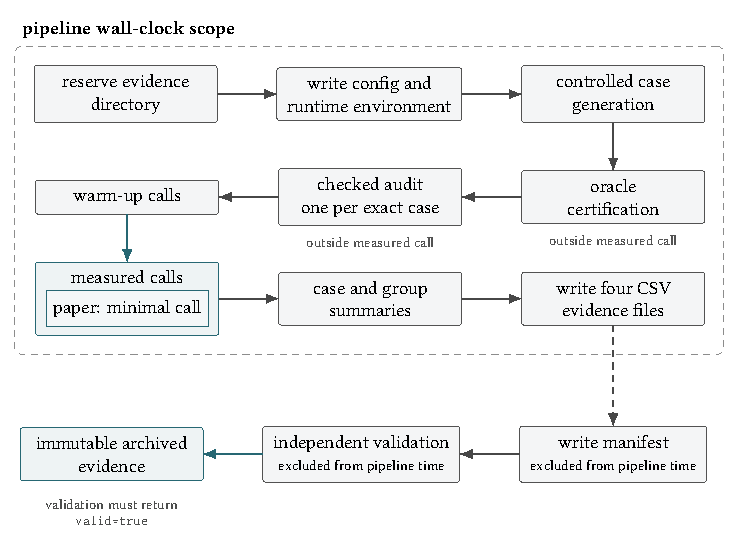
\includegraphics[width=.94\textwidth]{formal_experiment_pipeline.pdf}
  \caption[Historical formal pipeline and timing scopes.]{Historical formal
  experiment. Oracle certification and checked audits precede warm-up; only
  the selected call is timed. The paper call uses the rollback-enabled
  \texttt{minimal} implementation. Pipeline wall time has a separate scope.}
  \label{fig:method-formal-pipeline}
\end{figure}

\subsection{Fail-Closed Validation}
\label{sec:method-validation}

The separate evidence validator reconstructs all 60 cases from the fixed
protocol and recomputes seeds, hashes, oracle validity and structural profiles.
It reruns checked diagnostics and compares outputs, processed counts, trace
counts and every recorded paper metric. It verifies the complete
case--algorithm--round product and positions, positive times, correctness,
schemas, counts, source/environment provenance, wall-clock consistency and
file hashes. Summaries are recomputed from the raw measurements.

Malformed or inconsistent evidence is rejected rather than authorized for
analysis. The archived report is retained, and analysis validates the evidence
again before using it. This checks the experiment's evidence contract; it
neither reruns the timed observations nor formally proves the algorithm.
The full field-level validation procedure remains in the versioned
reproduction materials.

\section{Interpretation Boundary}
\label{sec:method-boundaries}

The conclusions concern the selected valid inputs, unequal family composition,
recorded versions and one environment. Repetition does not enlarge the input
sample; five sizes do not establish asymptotic complexity. Historical
paper/reference ratios retain their different-call-scope interpretation, and
counter associations remain descriptive. \Cref{chap:limitations} develops
these limitations rather than treating the archived study as current-backend
or hardware-independent evidence.
